
\chapter{Current System and Proposals, Requirements and Design of New System}\label{sec:currentsystemandproposals}

\section{Current System}
This section is intended to give some statistics and briefly discuss design of the current system. Table~\ref{table:currentstats} gives statistics 
of current system.
\begin{table}
\centering
\begin{tabular}{|c|c|}
\hline Number of experts & 1569 \\
\hline Number of publications UK & 22225 \\
\hline Number of all documents   & 24823 \\ 
\hline Number of tokens (terms) & 6876832 \\
\hline
\end{tabular}
\caption{Statistics of Current System} \label{table:currentstats}
\end{table}

\begin{figure}
 \centering
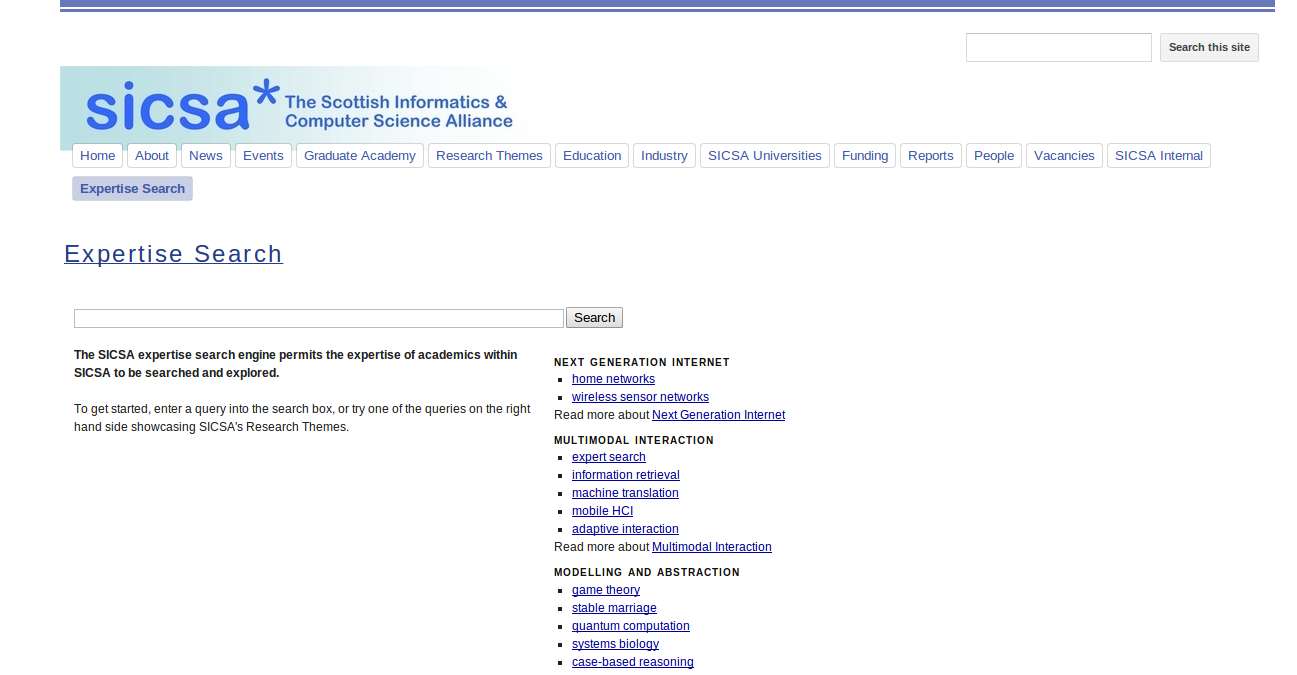
\includegraphics[width=13cm,height=15cm,keepaspectratio]{./figures/oldsicsa.png}
 \caption{Home Page} \label{fig:oldsicsa} 
 \end{figure}
 \begin{figure}
 \centering
 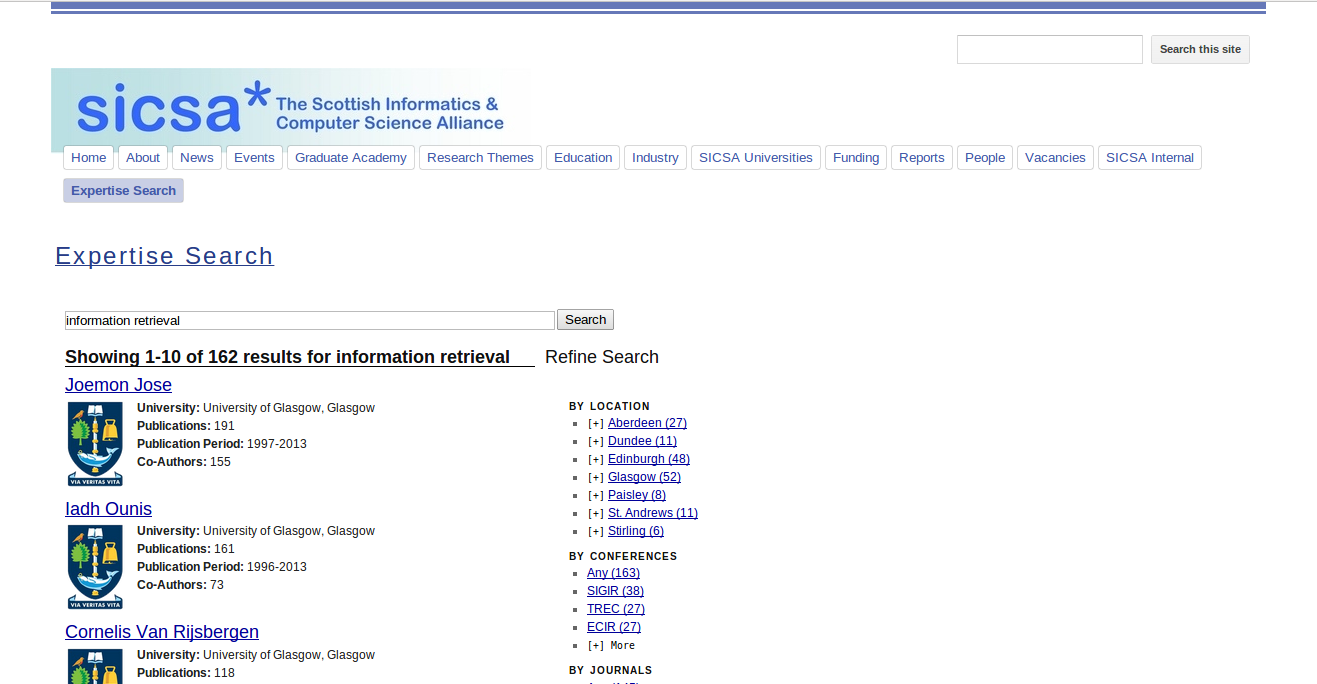
\includegraphics[width=13cm,height=15cm,keepaspectratio]{./figures/oldsearch.png}
 \caption{Experts In Response to ``information retrieval'' Query} \label{fig:resultspage} 
 \end{figure}
 \begin{figure}
 \centering
 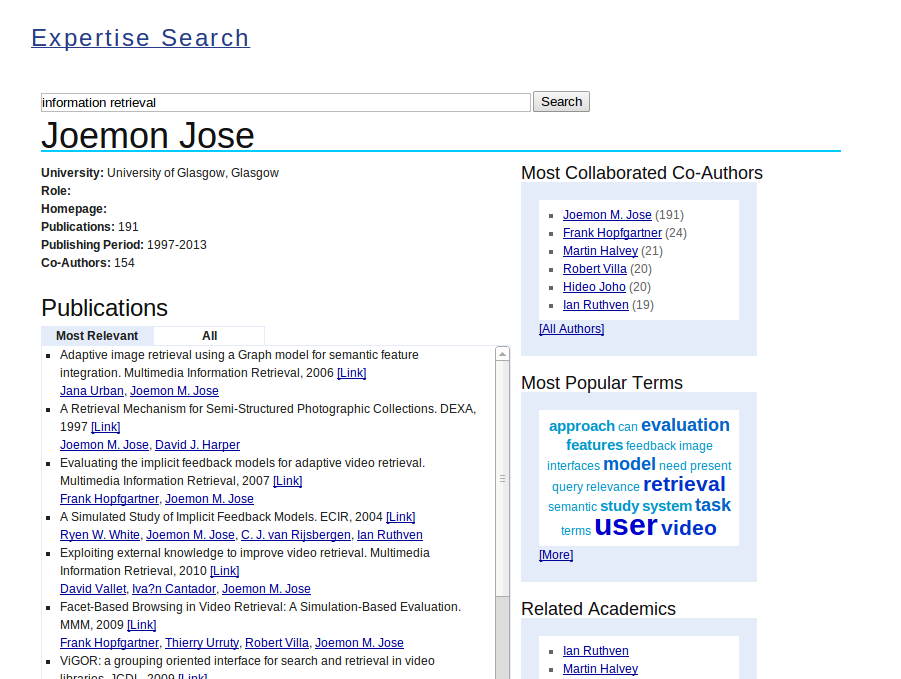
\includegraphics[width=13cm,height=15cm,keepaspectratio]{./figures/oldProfilePage.png}
 \caption{Old Expert's Profile Facet} \label{fig:profilepage} 
\end{figure}
Figure~\ref{fig:oldsicsa} is the home page of SICSA. It provides a set of sample queries categorised in 4 different categories on the right of the 
search panel. The top panel shows links to different SICSA pages. The middle panel is the search panel. It is independent of other panels. 
Experts (results) with respect to a query are independently shown in this panel without reloading other panels. Figure~\ref{fig:resultspage} shows
the interface when experts with respect to a query, ``information retrieval'' are shown. Also, the system demonstrates 
faceted search for academics by presenting refinement options using university, location and total publication range categories.
Below the refinement options is popular tags (terms) appear in expert's profiles the system retrieved.
Each result in the search panel includes expert's details: university, number of publications, publication period and total number of coauthors.

Figure~\ref{fig:profilepage} illustrates a profile page of an expert. This page introduces most collaborated coauthors facet on the right of the page, a 
facet that shows popular terms appearing in an expert's profile and publications and related academics facet.

\paragraph{Design and Architecture of Current System}

 \begin{figure}
 \centering
 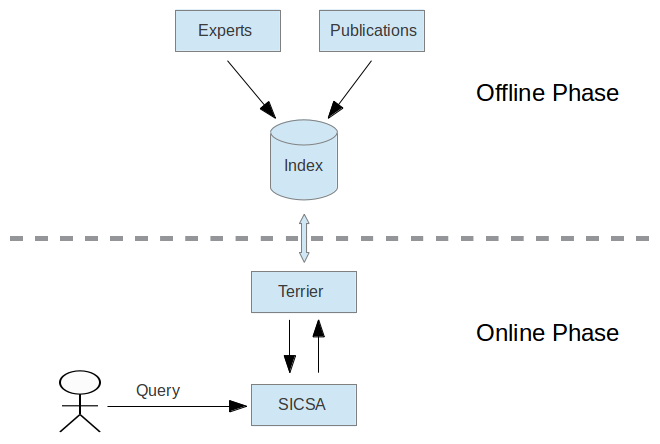
\includegraphics[scale=0.5,keepaspectratio]{./figures/currentSystemDesign.jpg}
 \caption{Design of Current System} \label{fig:currentDesign} 
\end{figure}
Figure~\ref{fig:currentDesign} shows design of current system. It makes use of publication as expertise. From the figure, after a user submits a query
to the system, the system sends a query to Terrier and finally Terrier returns relevant experts to the user.

\section{Expert Search Indicators of New System}\label{section:goodexpert}
In section~\ref{sec:presentingQueryResult}, it was obvious that some evidence could be used to convince users how reliable a document (link) is.
In this secion, the evidence within
the context of this project will be discussed. As discussed in section~\ref{section:aims}, this project makes use of publications and funded projects as 
expertise evidence. Based on these evidence, what makes an expert a good expert? we propose several intuitions about a relevant expert as follows 
\begin{itemize}
 \item he has published a lot of publications.
 \item he has co-authored with a lot of other experts in publications.
 \item he has co-authored with a lot of other experts in funded projects.
 \item he has received a lot of funding.
 \item he has involved in a lot of projects.
\end{itemize}

It can be seen clearly that these assumptions or features in learning to rank are independent of the query a user submits. These features are query independent
(section ~\ref{section:queryindependent}). However, query dependent features (section~\ref{section:querydependent}) should take into account as well. 
In this project, there are 2 query dependent features: 
\begin{itemize}
 \item funded projects feature
 \item publication features feature
\end{itemize}

To sum up, a good expert should have high scores in both query dependent and independent features.

\subsection{Requirements Specification}
Due to the scope of the project it would be impossible to start without a clear vision of how
the end product should function. These requirements were decided on during the early stages of the project. 
The reasoning behind them comes primarily from a number of sources:
\begin{itemize}
 \item Research into a previous attempt at current SICSA system (section~\ref{sec:currentsystem}).
 \item Research into presenting query results (section~\ref{sec:presentingQueryResult}).
 \item Research into learning to rank techniques to enhancing the performance of the retrieval system by integrating different kinds of 
 expertise evidence (section~\ref{sec:letor}).
 \item Discussion with Dr. Craig Macdonald.
\end{itemize}
% However, developing an IR system is researched based. Utilizing learning to rank technique might not 
% produce optimal ranking due to the lack of training dataset. Therefore, 
The requirements have been split into 2 sections depending on their necessity: functional requirements and non-functional requirements

\paragraph{Functional Requirements}
\subsubsection{Must Have}
\begin{itemize}
 \item Extracting funded projects from 2 different sources: Grant on the Web~\cite{gow} and Research Councils UK~\cite{gtr}.
 \item Integrating publications and funded projects as expertise evidence.
 \item Utilizing learning to rank techniques with an attempt to enhance the performance of the retrieval system.
 %\item Indexing and Retrieving documents (experts) effectively.
 \item Able to conclude that applying learning to rank techniques helps improve the performance of the retrieval system using evaluation matrics discussed
 in section~\ref{sec:evaluation}. 
\end{itemize}

\subsubsection{Should Have}
\begin{itemize}
 \item providing refinement options for users to filter results by funded projects, publications and both.
 \item providing refinement options for users to filter funded projects and publications of each expert.
\end{itemize}

\subsubsection{Could Have}
\begin{itemize}
 \item not yet
\end{itemize}

\subsubsection{Would Like to Have}
\begin{itemize}
 \item Ability to upload funded projects manually by members of the system.
\end{itemize}

\paragraph{Non-functional Requirements}
\begin{itemize}
 \item Functional 24 hours a day.
 \item Update data regularly.
 \item Able to load all evidence into main memory for efficient lookup.
 \item Fully functional for the purpose of the final demonstration.
\end{itemize}

\subsection{Design and Architecture of New System} \label{section:union}
Figure~\ref{fig:newDesign} shows design of new system. It makes use of learning to rank (LETOR) technique to integrate 
both publication and funded projects as expertise evidence. From the figure, the design is quite similar except that query results (experts) are
applied with learning to rank technique to obtain optimal ranking.

 \begin{figure}
 \centering
 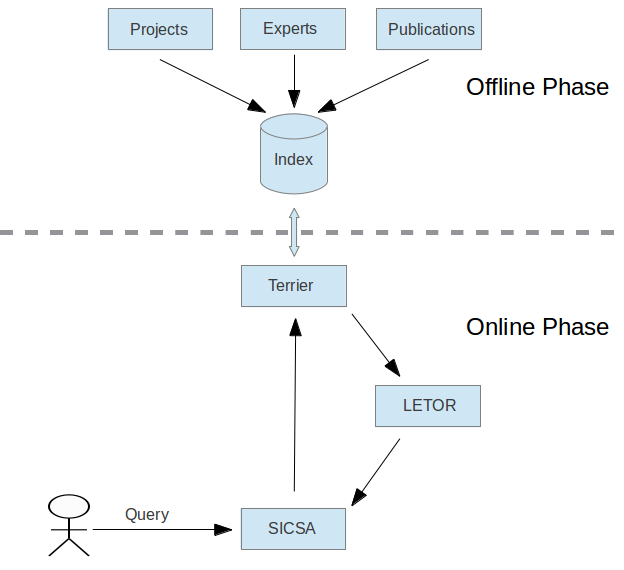
\includegraphics[scale=0.5,keepaspectratio]{./figures/newSystemDesign.png}
 \caption{Design of Current System} \label{fig:newDesign} 
\end{figure}

\paragraph{Retrieving Documents (Experts) with Respect to a Query} 

\begin{figure}
\centering
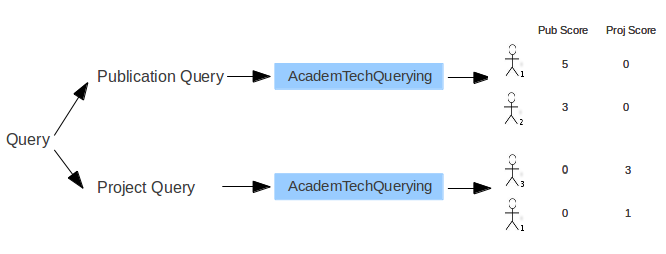
\includegraphics[scale=0.7]{./figures/querying.png}
\caption{Querying} \label{fig:quering} 
\end{figure}
\quad
\begin{figure}
\centering
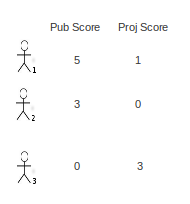
\includegraphics[scale=0.7]{./figures/union.png}
\caption{Results After Union} \label{fig:union} 
\end{figure}
In the previous section, we gave a broad view of the new system retrieval scheme. In this section, we will be more specific on how we are going to 
obtain results from user query and apply them to learning to rank technique to obtain optimal ranking.
Figure~\ref{fig:quering} shows the process of obtaining documents (experts) with respect to a query. 

Given a query $Q$, it is transformed into publication query $Q_{pub}$, using only publications as expertise evidence and project
query $Q_{proj}$, using only funded projects as expertise evidence. 
AcademTechQuerying Class then processes both $Q_{pub}$ and $Q_{proj}$. The results of both
queries are then unioned, denoted $R_{pub,proj}(Q)$ as shown in Figure ~\ref{fig:union}. The results obtained are based on query dependent features as discussed in section 
~\ref{section:querydependent}. Finally, unioned results are applied to a learned model to generate optimal ranking. Next section will discuss more in
details.
